\documentclass[a4paper,10pt]{article}
%\usepackage{anysize}
%\marginsize{2cm}{2cm}{1cm}{1cm} 
\usepackage{xltxtra}
\usepackage{xunicode}
\usepackage{graphicx}
\usepackage{color}
\usepackage{xgreek}
\usepackage{fancyvrb}
\usepackage{minted}
\usepackage{listings}
\usepackage{enumitem} 
\usepackage{framed} 
\usepackage{relsize}
\usepackage{float} 
\setmainfont[Mapping=tex-text]{FreeSerif}
\begin{document}

\def\thesubsection {Άσκηση (\roman{subsection})}

\begin{titlepage}
\begin{center}
\begin{figure}[h] 
     
\includegraphics[width=0.2\textwidth]{title/ntua_logo}
\end{figure}
\vspace{1cm}
\begin{LARGE}\textbf{ΕΘΝΙΚΟ ΜΕΤΣΟΒΙΟ ΠΟΛΥΤΕΧΝΕΙΟ\\[1.5cm]}\end{LARGE}
\begin{Large}
ΣΧΟΛΗ ΗΜ\&ΜΥ\\
Συστήματα Μικροϋπολογιστών\\[2cm]
1\textsuperscript{η} Άσκηση\\
Ακ. έτος 2011-2012\\
\end{Large}
\vfill
\begin{flushright}
\begin{tabular}{l r}
{Γρηγόρης \textsc{Λύρας}}&
{Α.Μ.: 03109687}\\
\end{tabular}
\end{flushright}

\large\today\\
\end{center}
\end{titlepage}




\section*{} 
\subsection{}

Στην άσκηση αυτή μας ζητείται να αποκωδικοποιήσουμε το πρόγραμμα που μας
δίνεται από γλώσσα μηχανής σε assembly. Από τη δοσμένη ακολουθία έχουμε τον
εξής κώδικα:
\noindent Κυρίως κώδικας:
\inputminted[linenos,obeytabs,fontsize=\footnotesize]{nasm}{files/1-1.8085}

Το πρόγραμμα αυτό παίρνει είσοδο από τα dip switches (2000H) και βρίσκει τη
θέση του πρώτου αναμένου bit από τα δεξιά. Τη θέση αυτή την εμφανίζει στα leds
(3000H) στο δυαδικό σύστημα. 

Για να έχουμε συνεχόμενη λειτουργία αρκεί το RST 1 στο τέλος του προγράμματος
να γίνει JMP START.

\subsection{}

Εδώ μας ζητείται να υποποιήσουμε ένα πρόγραμμα ανάβει κυκλικά με χρονική
καθυστέρηση 0.5 sec. Αν ο δεξιότερος διακόπτης στα dip switches είναι ON τα 
leds ανάβουν από τα δεξιά προσ τα αριστερά και αντίστροφα. 

\noindent Κυρίως κώδικας:
\inputminted[linenos,obeytabs,fontsize=\footnotesize]{nasm}{files/1-2.8085}

\subsection{}

Το πρόγραμμα που υλοποιούμε μετατρέππει τον αριθμό που διαβάζει από τα dip
switches στη δεκαδική του μορφή και τον εμφανίζει στα leds, με τις δεκάδες να
απεικονίζονται στα 4 MSB και τις μονάδες στα 4 LSB.  Για να έχουμε συνεχή
λειτουργία χρησιμοποιούμε το JMP START. Αν ο αριθμός της εισόδου είναι
τριψήφιος ανάβουν όλα τα leds.

\noindent Κυρίως κώδικας:
\inputminted[linenos,obeytabs,fontsize=\footnotesize]{nasm}{files/1-3.8085}

\subsection{}
Σε αυτή την άσκηση καλούμαστς να υλοποιήσουμε το κύκλωμα που μας δίνεται. Η
είσοδος δίνεται από τα dip switches, και η έξοδος εμφανίζεται στα leds. Το
πρόγραμμα έχει συνεχή λειτουργία.

\noindent Κυρίως κώδικας:
\inputminted[linenos,obeytabs,fontsize=\footnotesize]{nasm}{files/1-4.8085}


\subsection{}
\subsubsection*{}
Τέλος έχουμε μια τεχνοοικονομική μελέτη με θέμα την κατασκευή μια φορητή
ηλεκτρονική συσκευή με χρήση 3 τεχνολογιών.

Τεχνολογίες:
\begin{itemize}
    \item Διακριτά στοιχεία και ολοκληρωμένα κυκλώματα σε πλακέτα
        \begin{equation}
            Cost=20000+(15+15)\times{x}=20000+30\times{x}
        \end{equation}
    \item FPGAs και λίγα περιφεριακά σε μικρότερη πλακέτα
        \begin{equation}
            Cost=10000+(60+10)\times{x}=10000+70\times{x}
        \end{equation}
    \item Σχεδίαση SoC για πολύ μικρή πλακέτα
        \begin{equation}
            Cost=300000+(1+1)\times{x}=300000+2\times{x}
        \end{equation}
\end{itemize}

\begin{figure}[H] 
     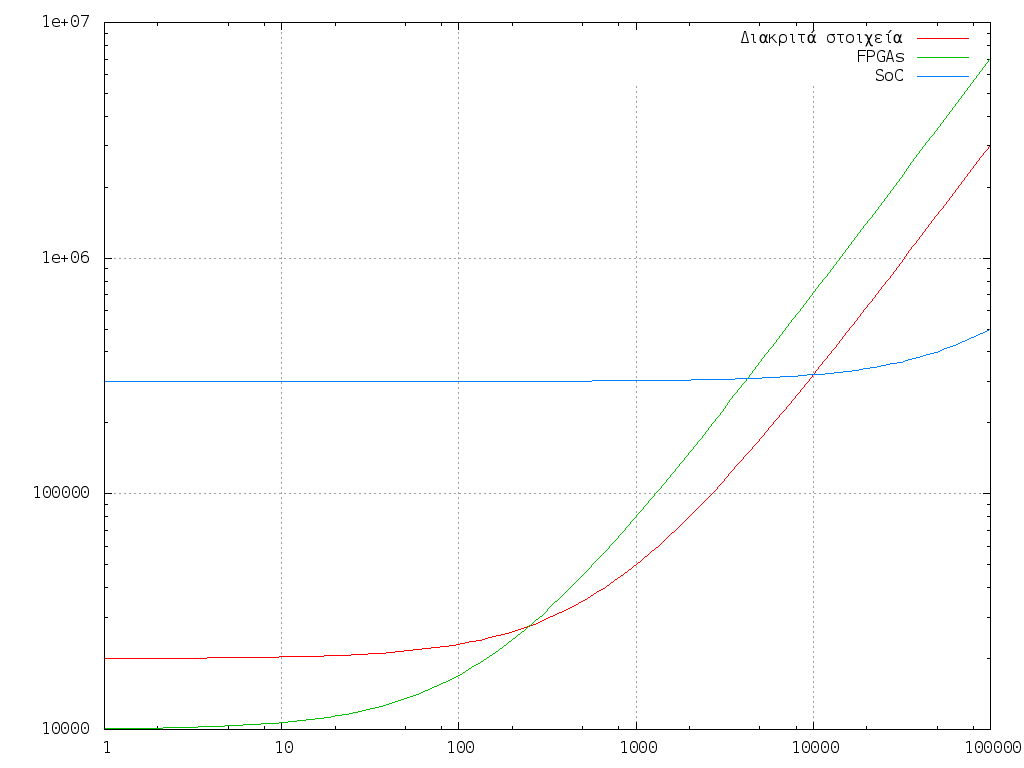
\includegraphics[width=0.9\textwidth]{files/plot1.png}
     \caption{Καμπύλες ανά τεμάχιο (λογαριθμική κλίμακα)}
\end{figure}
Για να είναι μη συμφέρουσα η επιλογή των FPGA θα πρέπει η τιμή των
ολοκληρωμένων για τα FPGA να ανέρχεται στα 20\euro.

\subsubsection*{}
Επαναλαμβάνοντας τους υπολογισμούς συνυπολογίζοντας στο κόστος και άλλους
συντελεστές για κάθε τεχνολογία (π.χ. κόστος μπαταρίας, αυτονομία, 
κατανάλωση, μέγεθος) έχουμε τα ακόλουθα.
Τεχνολογίες:
\begin{itemize}
    \item Διακριτά στοιχεία και ολοκληρωμένα κυκλώματα σε πλακέτα
        \begin{equation}
            Cost=20000+(15+15)\times{x}=20000+30\times{x}
        \end{equation}
    \item FPGAs και λίγα περιφεριακά σε μικρότερη πλακέτα
        \begin{equation}
            Cost=0.8\times{(10000+(60+10)\times{x})}=\times{(10000+70\times{x})}
        \end{equation}
    \item Σχεδίαση SoC για πολύ μικρή πλακέτα
        \begin{equation}
            Cost=0.7\times{(300000+(1+1)\times{x})}=0.7\times{(300000+2\times{x})}
        \end{equation}
\end{itemize}

\begin{figure}[H] 
     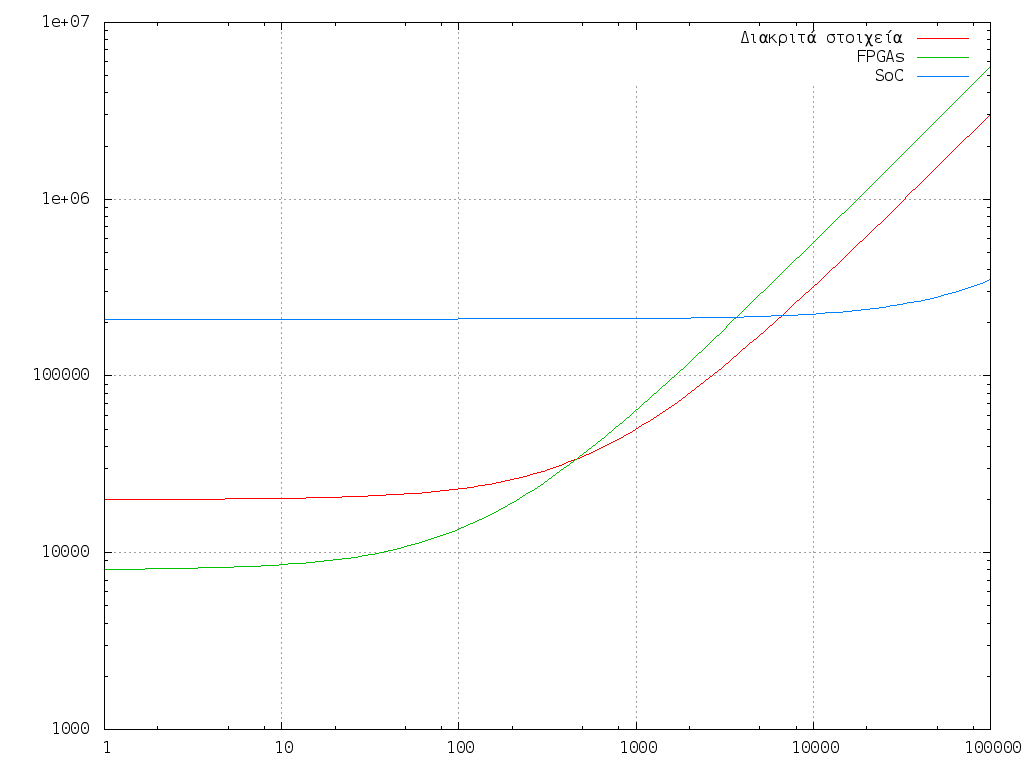
\includegraphics[width=0.9\textwidth]{files/plot2.png}
     \caption{Καμπύλες ανά τεμάχιο (λογαριθμική κλίμακα)}
\end{figure}



\end{document}
